\documentclass[11pt]{exam}
\usepackage{epsfig}

\usepackage{hyperref}
\usepackage{enumitem}
\usepackage[centertags]{amsmath}
%\usepackage{amsfonts}
\usepackage{amssymb}
\usepackage{amsthm}
\usepackage[all]{xy}
\usepackage{newlfont}
\usepackage{amsmath,amssymb,bm,mathtools}

\usepackage{xcolor} %for color
\usepackage{xmpmulti}
%\usetheme{Air}
%\usefonttheme{professionalfonts}
\usepackage{thumbpdf}
\usepackage{wasysym}
\usepackage{upgreek}
\usepackage{ucs}
%\usepackage[utf8]{inputenc}
\usepackage{pgf,pgfarrows,pgfnodes,pgfautomata,pgfheaps,pgfshade}
\usepackage{verbatim}
\usepackage{empheq}
\newcommand*\widefbox[1]{\fbox{\hspace{2em}#1\hspace{2em}}}

\newcommand{\Integer}{\mathbb{Z}}
\newcommand{\Natural}{\mathbb{Z}_{\geq 0}}
\newcommand{\Naturalstar}{\mathbb{Z}_{> 0}}
\newcommand{\Real}{\mathbb{R}}
\newcommand{\Complex}{\mathbb{C}}
\newcommand{\hilbert}{\mathcal{H}}
\newcommand{\BigHilbert}{\bm{\mathcal{H}}}
\newcommand{\innprod}[2]{\langle{#1},{#2}\rangle}
\newcommand{\ginnprod}[2]{\langle\!\langle{#1},{#2}\rangle\!\rangle}
\newcommand{\norm}[1]{\|{#1}\|}
\newcommand{\mrm}[1]{{\mathrm #1}}
\newcommand{\gnorm}[1]{|\!|\!|{#1}|\!|\!|}
\newcommand{\expect}{\mathbb{E}}

\newcommand{\gr}{\selectlanguage{greek}}

\newtheorem{definition}{Definition}

%\newcommand{\red}{\color{myred}}
%\newcommand{\blue}{\color{myblue}}
%\newcommand{\black}{\color{myblack}}


%\definecolor{BrickRed}{cmyk}{0,0.89,0.94,0.28}
%\definecolor{pink}{RGB}{255,192,203}

\begin{document}
\centerline{\Large \sc Homework 4 - Midterm 1. \underline{\textbf{DUE OCT 6th 11:59 PM}}}
\pagestyle{empty}

\hrulefill

\vspace{2cm}


{\Large \sc Name:}



\vspace{2cm}



{\Large \sc Student ID:}

\vspace{6cm}

\begin{itemize}
  \item Reasoning and work must be shown to gain partial/full
  credit
  \item Please include the cover-page on your homework PDF with your name and student ID. Failure of doing so is considered bad citizenship. 

 \end{itemize}

\clearpage
%{\bf Homework instructions}: You need to solve either question 1 or question 2, and you need to solve question 3. The total homework score will be the average given to two questions, either question 1 or 2, and that of question 3. You can solve the three questions if you wish; in the case of the two, I will choose the one that has the highest score. 
\section*{Maximum Matching}
 In order to solve this problem, we need to elaborate on how to use optimization of network flows, discussed in Lecture 4, to solve matching problems. The definition of {\it matching} is as follows:
 \begin{definition}{Matching}
 A matching ${\cal M}\subset {\cal E}$ is a subset of edges in a graph ${\cal G}=({\cal V},{\cal E})$ such that no two edges have vertexes in common. 
 The {\bf Maximum Matching} is the largest set ${\cal M}$ that is a matching set. This set is not unique in general. 
 \end{definition}
In bipartite graphs ${\cal G}=({\cal A}\cup {\cal B},{\cal E})$ the maximum matching set is useful to allocate, for instance, individual workers in ${\cal A}$ to individual tasks in ${\cal B}$, as shown in the figure:
\begin{center}
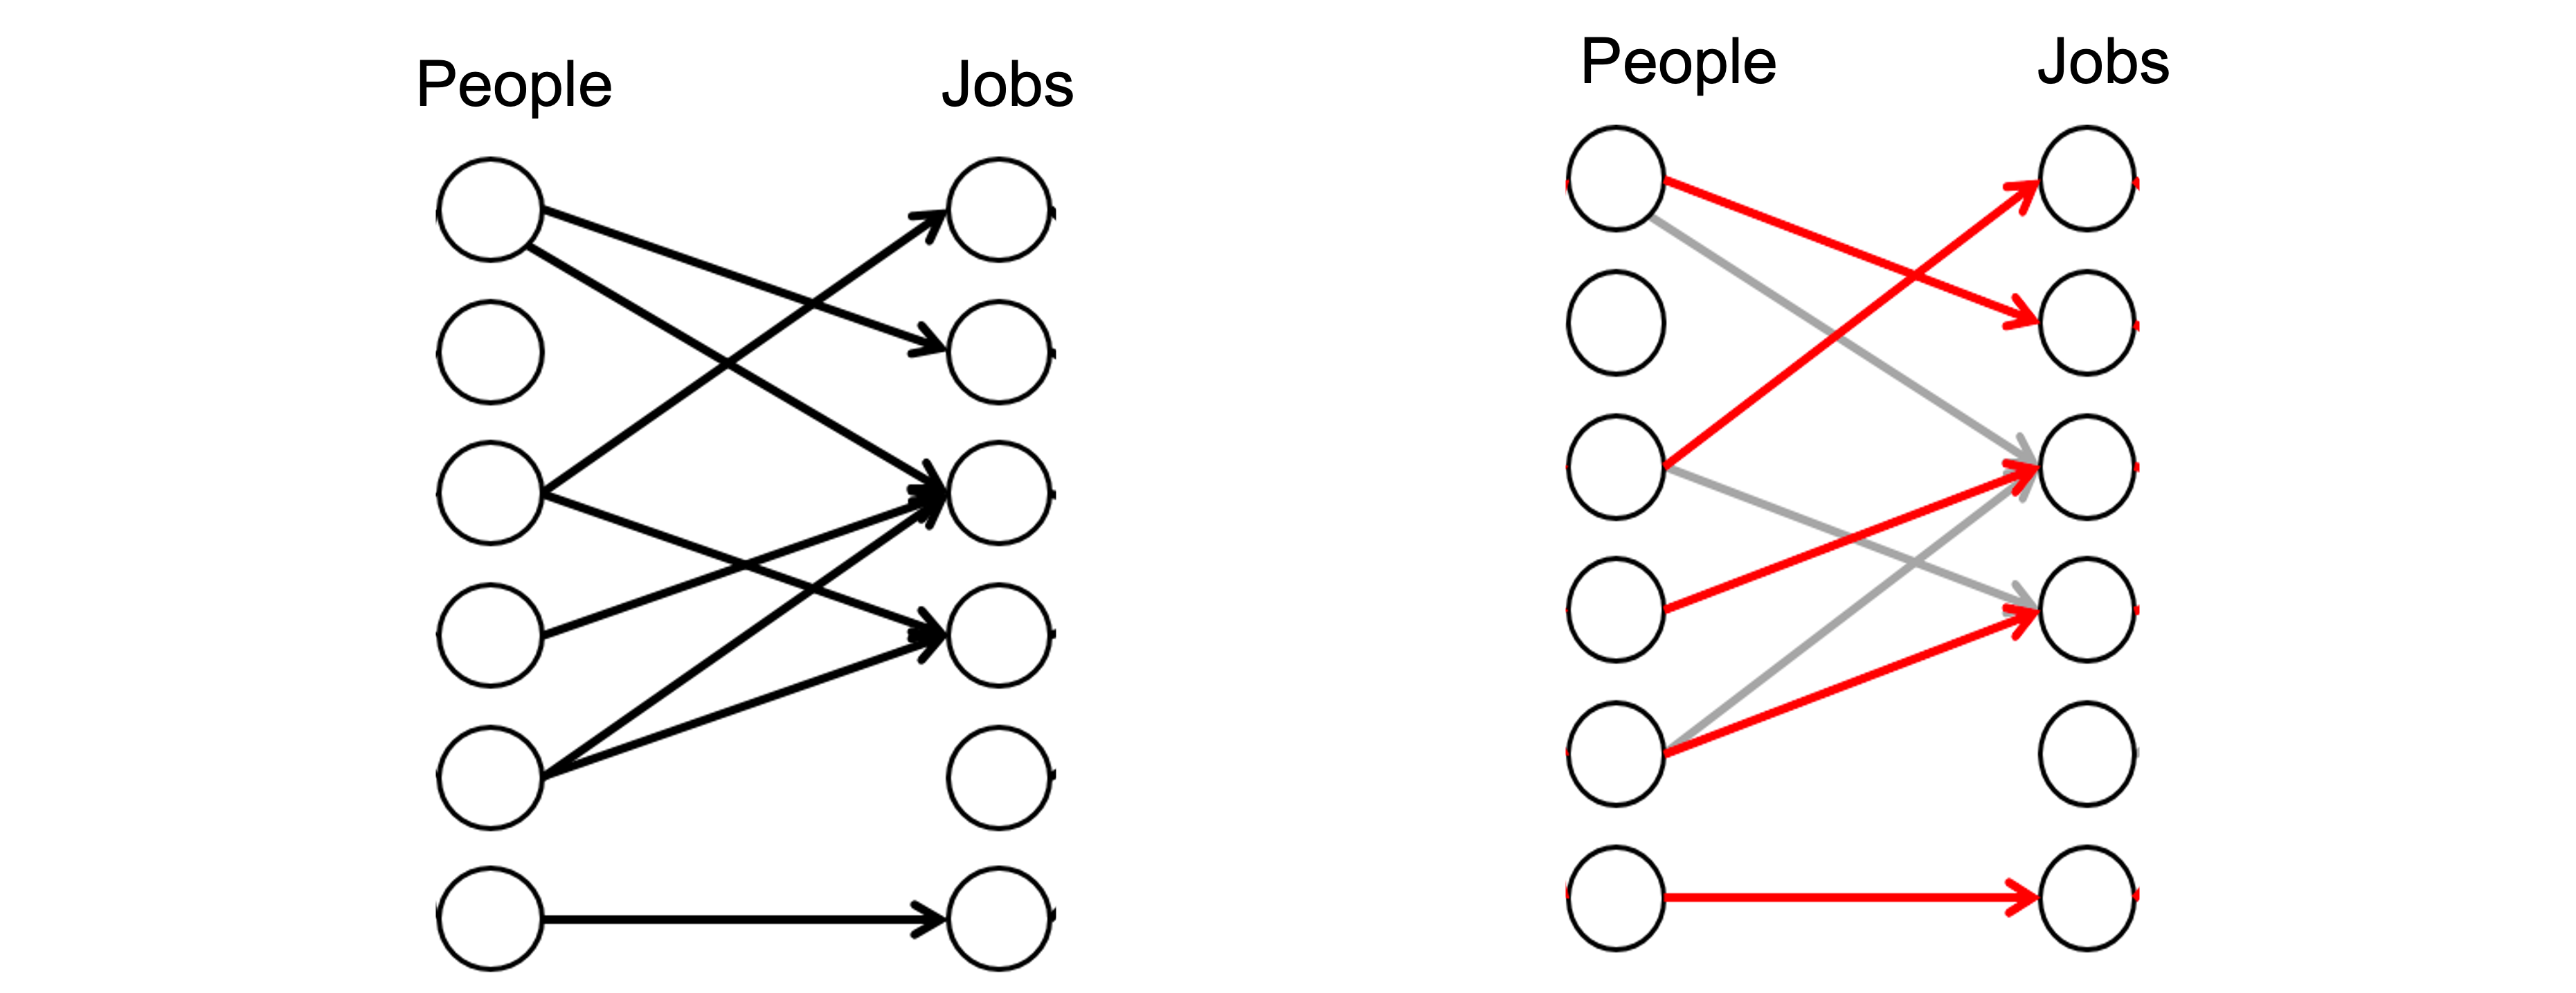
\includegraphics[width=0.8\linewidth]{people_jobs.png}
\end{center}
There are two interesting problems. 

\begin{enumerate}
\item One is finding such matching for the case where the workers are equally qualified to do the job; this amounts to finding the {\bf maximum matching}. This problem can be solved through a {\it max-flow} optimization, using the Ford-Fulkerson algorithm (in Python \texttt{networkx.maximum\_flow}). 
 \item The second one is finding an optimum match when the workers are {\it not equally qualified} to perform each job. In this case, not everyone can always pick the best for the task, so one way of addressing this problem is to maximize the average competence over all jobs. This problem can be mapped onto the so-called max-flow/min-cost problem, which uses the so-called {\it simplex method} (in Python \texttt{networkx.max\_flow\_min\_cost}). 
\end{enumerate}
The numerical methods to solve them are explained, respectively, in the next two sections. 
\subsection*{1. Solving the maximum matching with max-flow}
A solution can be obtained by converting the graph to a flow network. To do this, 
\begin{enumerate}
  \item Convert the graph edges to a directed edges going from $\cal A$ to $\cal B$. 
  \item Add a source node $s$ and a destination node $t$. 
  \item Draw edges from  $s$ to each node in $\cal A$ and from each node in $\cal B$ to $t$. 
  \item Set capacity $\overline{f}_{a,b}=1$ for each edge in the new graph.
\end{enumerate}
It can be shown that the max-flow solution of this flow network gives a maximum matching (might not be unique). The maximum flow equals the min-cut cardinality, which is going to be $\min(|{\cal A}|,|{\cal B}|)$.
\begin{center}
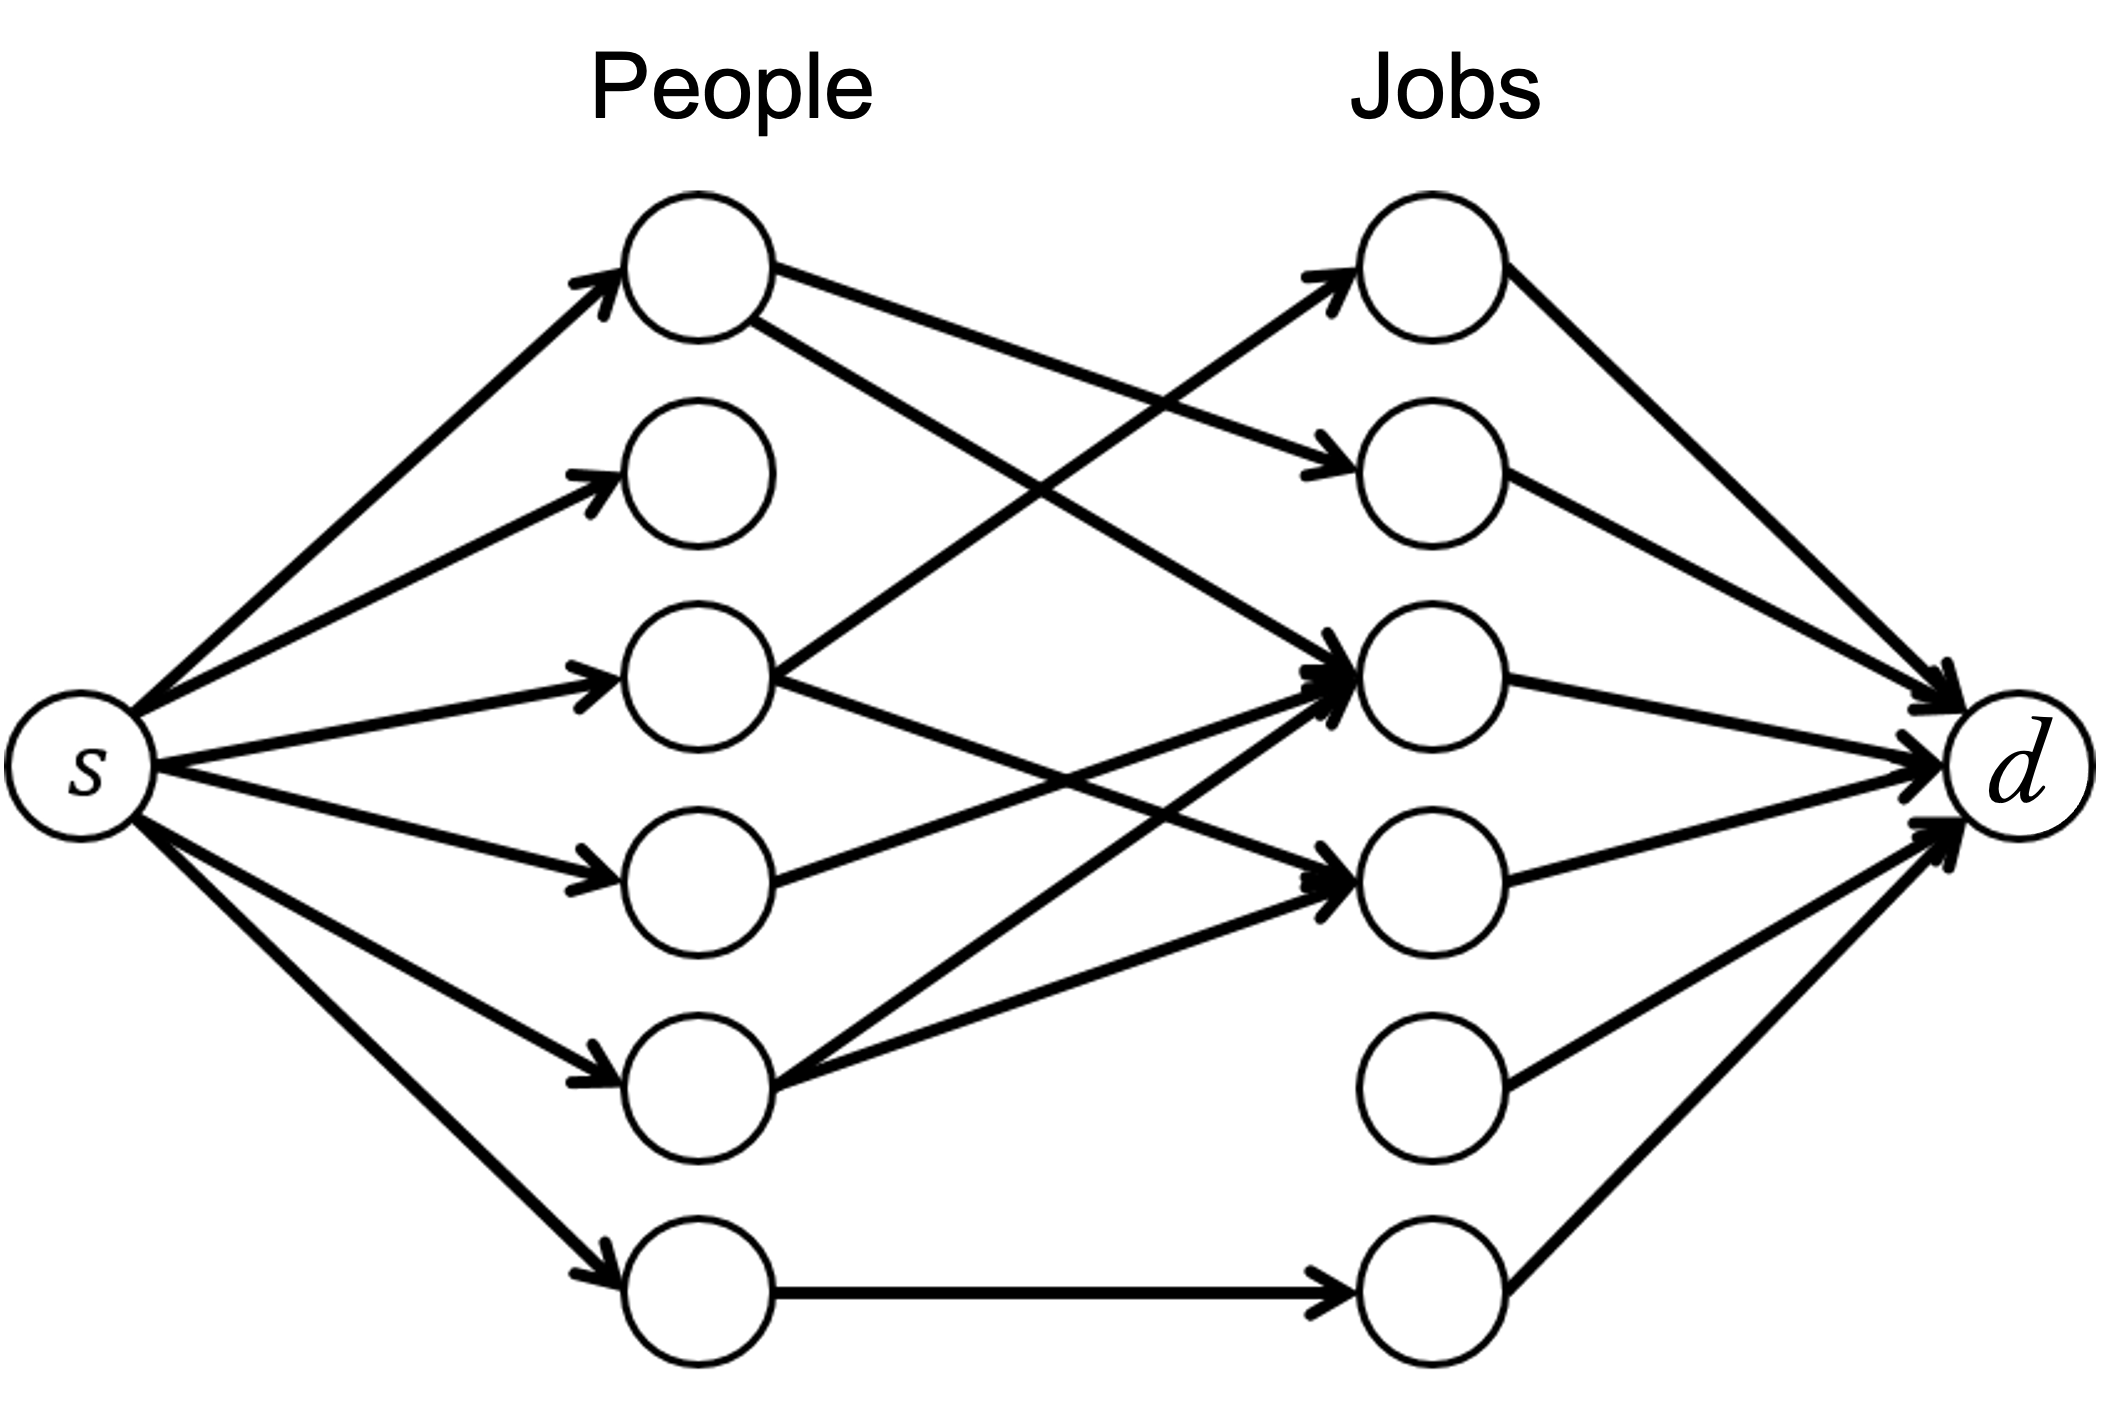
\includegraphics[width=0.4\linewidth]{bipartite-match1.png}
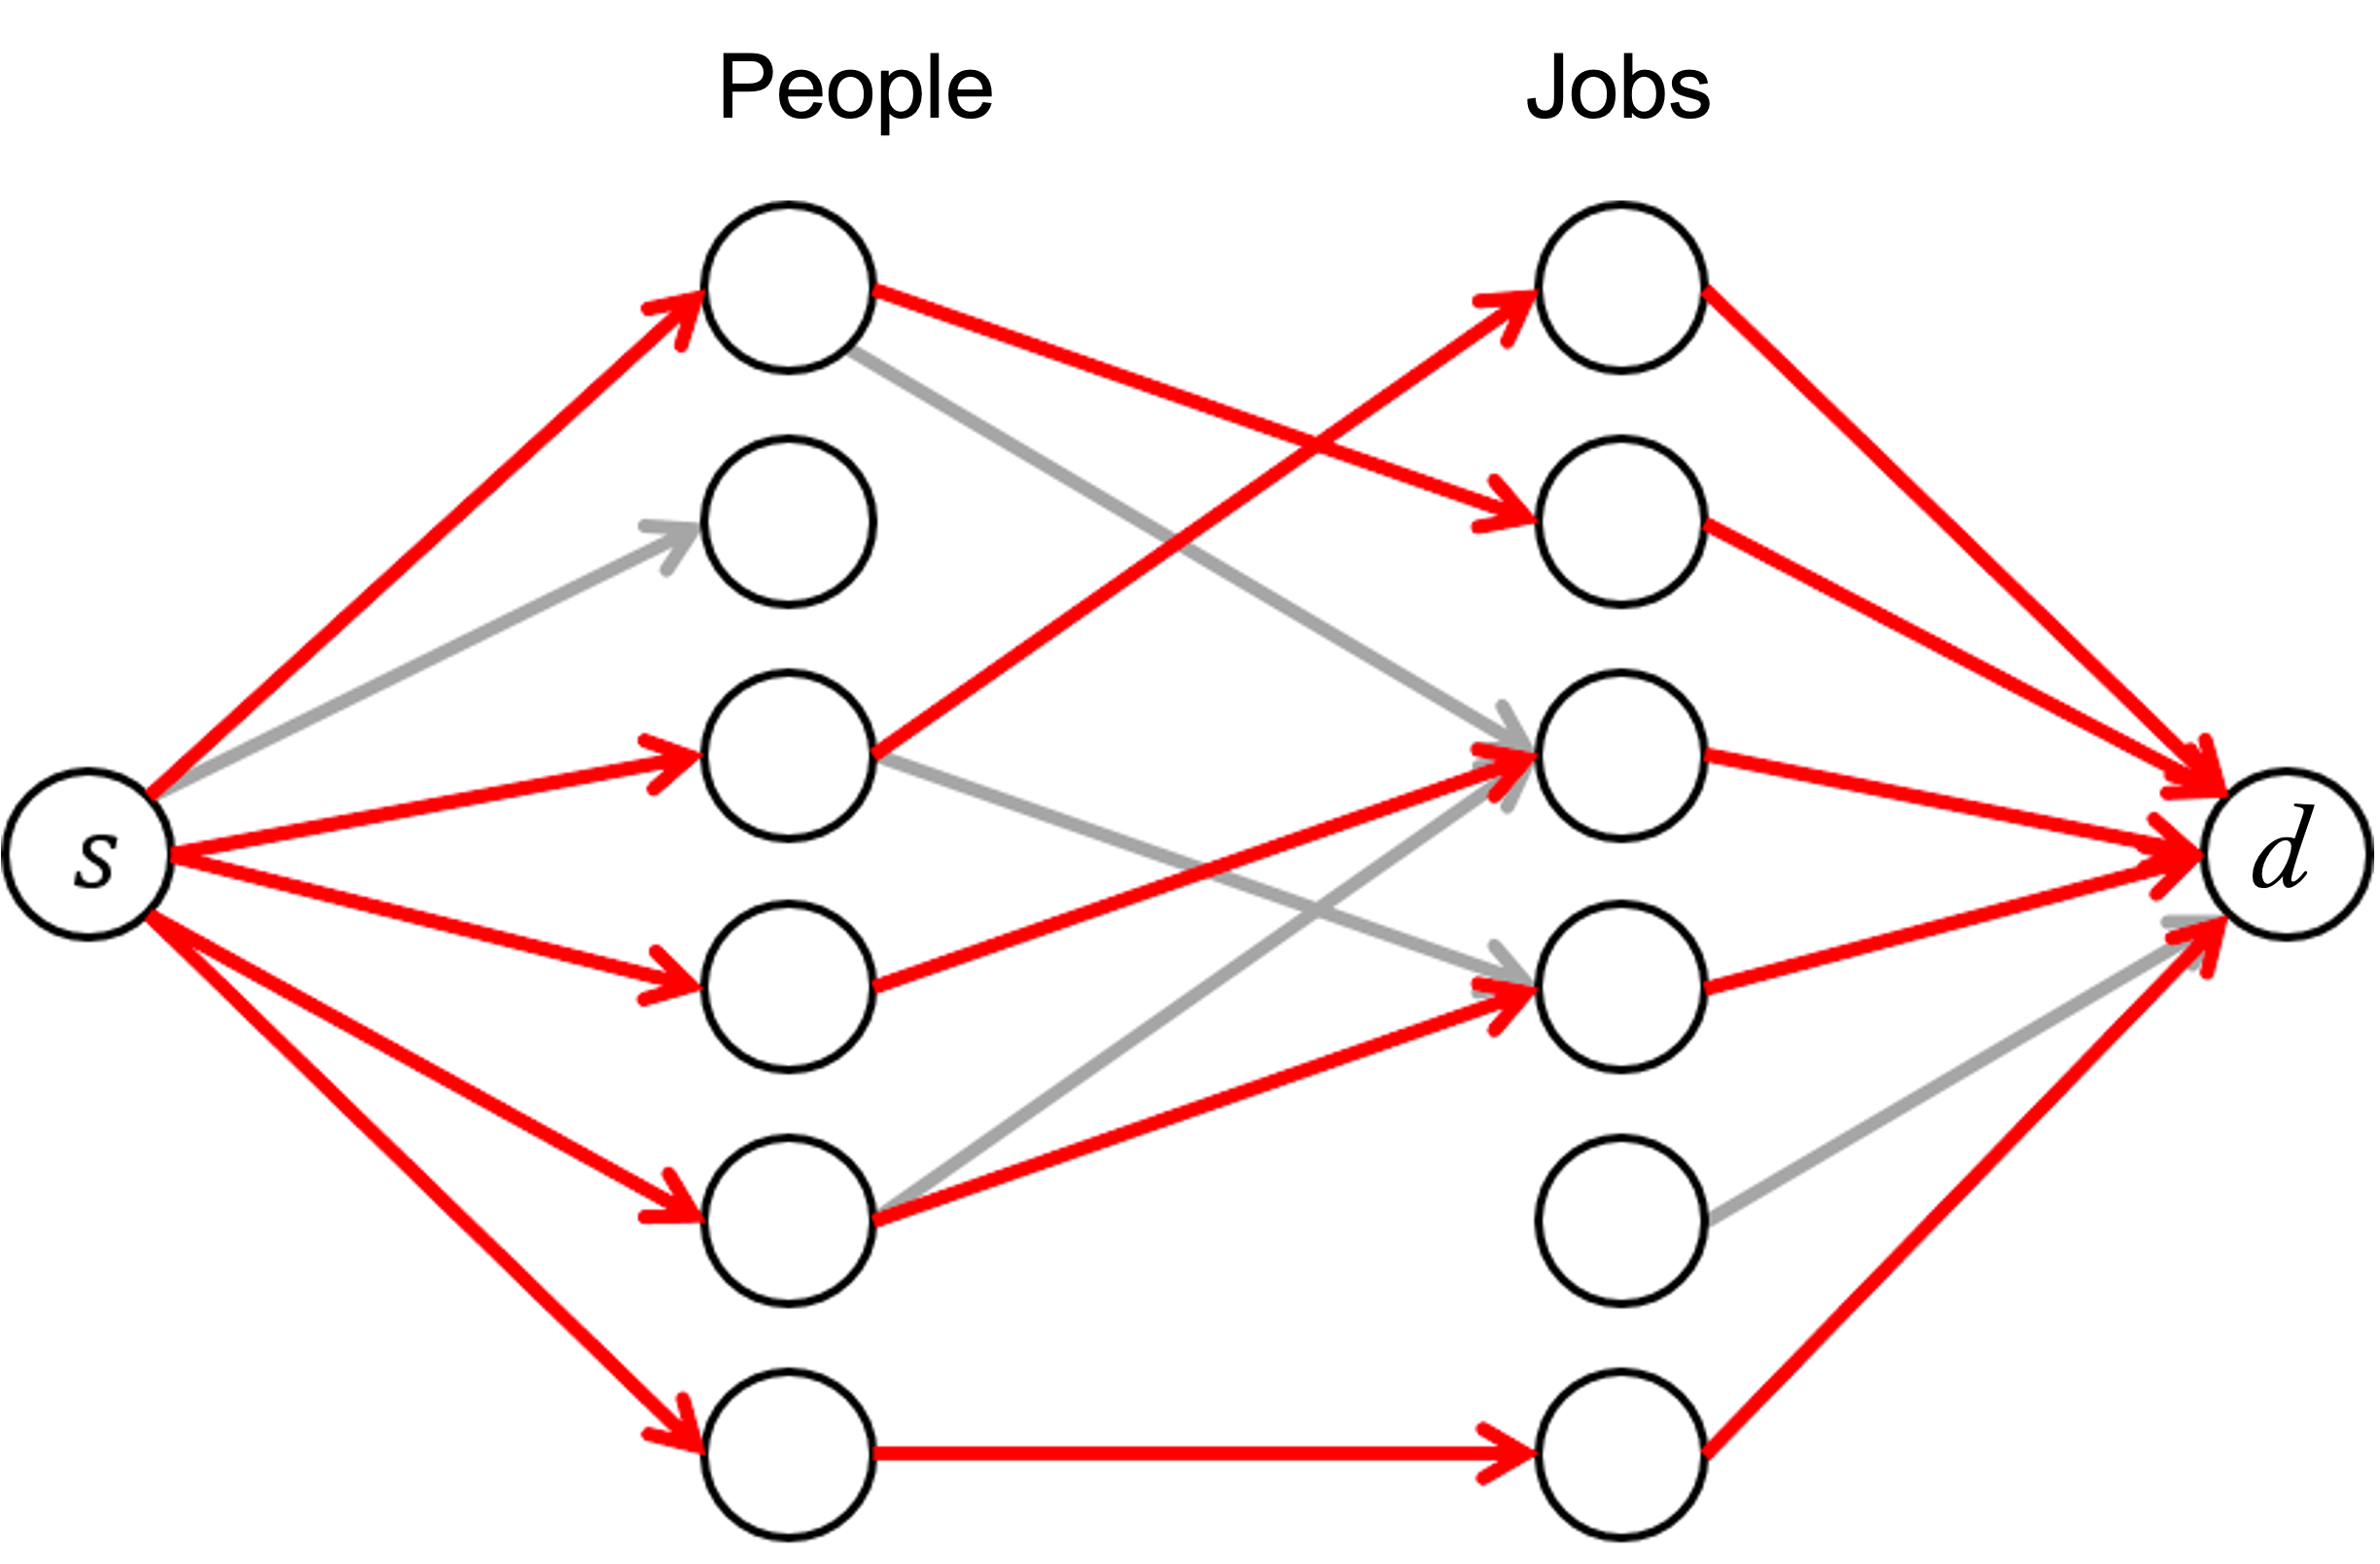
\includegraphics[width=0.4\linewidth]{bipartite-match2.png}
\end{center}
%
\subsection*{2. Solving for the minimum cost or maximum utility matching}
For the worker/job assignment problem, suppose the edge weight $w_{ab}$ is the {\it competence} of worker $a \in \cal A$ to perform job $b \in \cal B$ or the {\it reward} for choosing the edge $(a,b)$ in the matching, and the cost is equal to $-w_{ab}$ and capacities $\overline{\bm f}=\bm 1$. The problem of finding a matching that minimizes the cost or maximizes the average competency is known {\it linear sum assignment problem}, and its integer formulation is as follows:
\begin{align}
\text{minimize} &~-\bm w^\top \bm f\\
\mbox{subject to}&~\bm f\leq \bm 1,\\ 
&~\bm B^{\text{u}}\bm f\leq 1,\\  
&~\bm f \in \{0,1\}^{|\cal E|}
\end{align}
where $\bm f \in \{0,1\}^{|\cal E|}$ is the integrality constraint, $\bm B^{\text{u}}$ is the unoriented incidence matrix of the bipartite graph\footnote{\tt nx.incidence\_matrix(G,oriented=False)} and the constraint $\bm B^{\text{u}}\bm f\leq 1$ ensures that at most one edge is picked for each node. 

Because the integer problem is hard to solve, we can build a flow network problem that is not an integer problem but gives the same solution. As before, in addition to creating a flow network with capacities equal to one (i.e. $\overline{\bm f}=\bm 1$), we use the edge cost equal to $-w_{ab}$, where we can assign zero costs $-w_{sa}=0$ and $-w_{bt}=0$ for the artificial edges we added from source $s$ to the nodes in ${\cal A}$ and from the nodes in ${\cal B}$ to the target $t$. For this network flow problem, we already know that the maximum flow $y_s=\min(|{\cal A}|, |{\cal B}|)$ since this is the maximum flow over the minimum cut. The following problem formulation solves the minimum cost max-flow problem, with $\bm B$ the oriented incidence matrix:
   \begin{align}
      \text{minimize} &~-\bm w^\top \bm f\\
      \mbox{subject to}&~\bm f\leq \bm 1,\\
      &~[\bm B\bm f]_s=-[\bm B\bm f]_t=\min(|{\cal A}|, |{\cal B}|),\\
      &~[\bm B\bm f]_u=0,~~u\neq \{s,t\}  
    \end{align}
The python function to solve this problem is \texttt{networkx.max\_flow\_min\_cost}.

With this in mind, you can now solve the following question. You need to simply understand that the formulation of the question is a special case of a matching problem and use the appropriate Python functions to solve them. 
 
\newpage
\begin{questions}
\question[1--4]{\bf Max-Flow for bipartite graphs}:{\it Python/NetworkX question}\\
The Davis Southern women social network is a dataset collected in the 1930s. It contains the observed attendance at 14 social events by 18 Southern women. It can be accessed on networkX using the {\tt networkx.davis\_southern\_women\_graph} generator.
\begin{parts}

\part Plot this graph in  a bipartite layout (e.g., the left figure on Page 35 in Lecture 3).
\part Plot the graph that links the women that have been in the same social event.\\ {\it Hint: If you look at Lecture 3 slide 42, you can understand that the off-diagonal non-zero entries of $\bm A^2$ are what you are looking for...}
\part Plot the graph of the social events where one or more guests were the same. 
\\ {\it Hint: same suggestion as the previous one.}
\part Suppose that instead of social events, in the ``Davis Southern Women Graph'' the events are individual parking spaces available for EV charging, and that each woman can reach the spaces at about the same time. Let the weight, $w_{ab}$, on edge $(a,b)$ indicate the distance to destination of woman $a$ from parking space $b$. 

By setting $w_{ab} = 1$ for all $(a,b) \in \cal E$, answer the following questions: 
\begin{enumerate}[label=(\roman*)]
\item Indicate the number of women that will not be able to park and charge their car. 
\item Convert the graph into a flow network using the steps highlighted in the introduction.
Set the capacity of all the new edges to 1 and their weights to 0. Plot the flow network. 
\item Find the maximum bipartite matching for this graph using the flow network from the previous step. 
\end{enumerate}
\item Generate random weights for each link between the women and the parking spaces. These represent the distances. You can use a Rayleigh distribution for each (woman, spot) pair in the edge set using the function \texttt{numpy.random.rayleigh}.
\begin{verbatim}
  import numpy
  scale = 1
  size = size = G.number_of_edges()
  distances = numpy.random.rayleigh(scale=scale, size = size)
\end{verbatim}
\begin{enumerate}[label=(\roman*)]
  \item Convert the graph into a flow network using the steps highlighted in the introduction.
  Set the capacity of all the new edges to 1 and their weights to 0.
  \item Find the maximum bipartite matching that minimizes the average of distances of the edges in it.\\
  \textit{Useful methods}: \texttt{networkx.max\_flow\_min\_cost}
\end{enumerate}

\end{parts}


\question[1--2]{\bf Spectral Clustering}:{\it Python/NetworkX question}\\
In this problem, we want to apply spectral clustering methods to the Davis Southern women social network. We want to find the groups of people that attend similar events (a group of friends). For this problem, use the bipartite graph {\bf only} ({\bf DO NOT} use the women's graph or the events' graph)
\begin{parts}
\part Calculate the degree of the women, and the degree of the events. What women have the most socially active life? What are the most popular events?
\part Compute the eigenvector centrality and the betweeness centrality of the graph. What do you observe?
\part Find the eigenvectors and eigenvalues of the Laplacian of the graph. Plot the eigenvalues in ascending order.
\part Use spectral clustering to cluster the network. Use three clusters and plot the results. ({\it Hint: You may want to use k-means to do the clustering. Also, please use a different color for each cluster. Below, you will find a solution to the clustering problem}). What do you observe? Comment your results
\begin{center}
  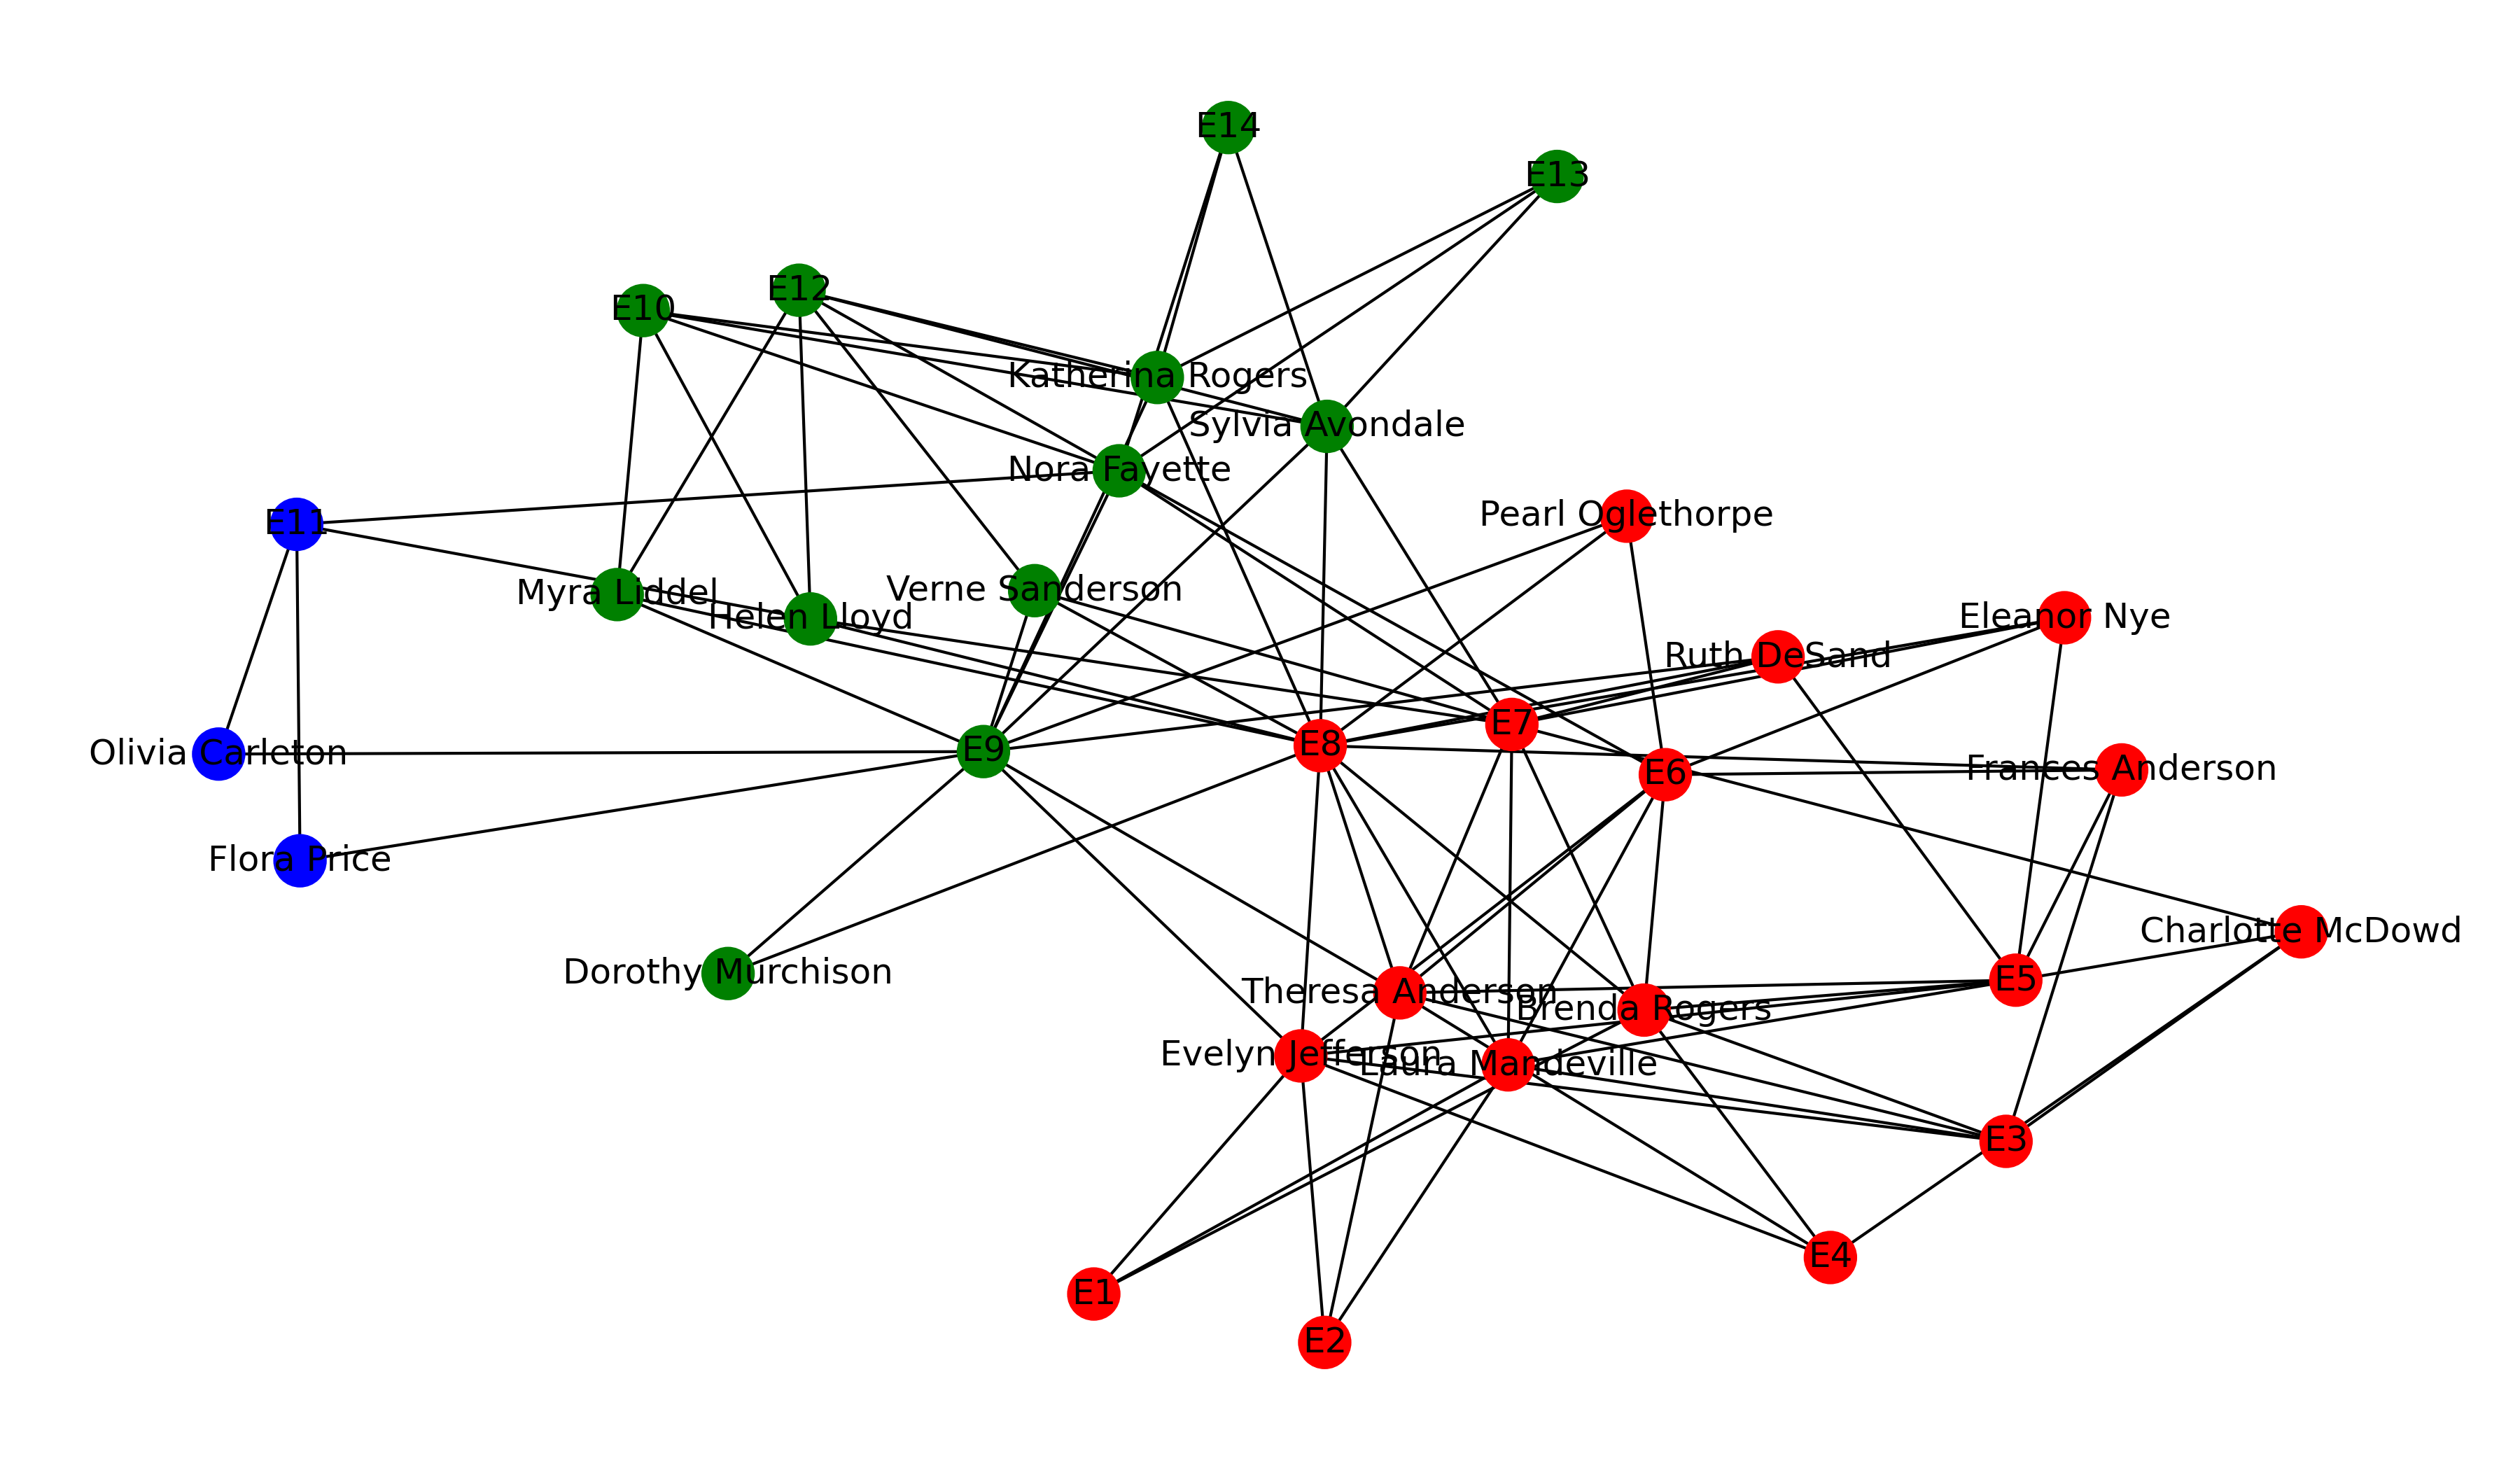
\includegraphics[width=0.8\linewidth]{cluster1.png}
  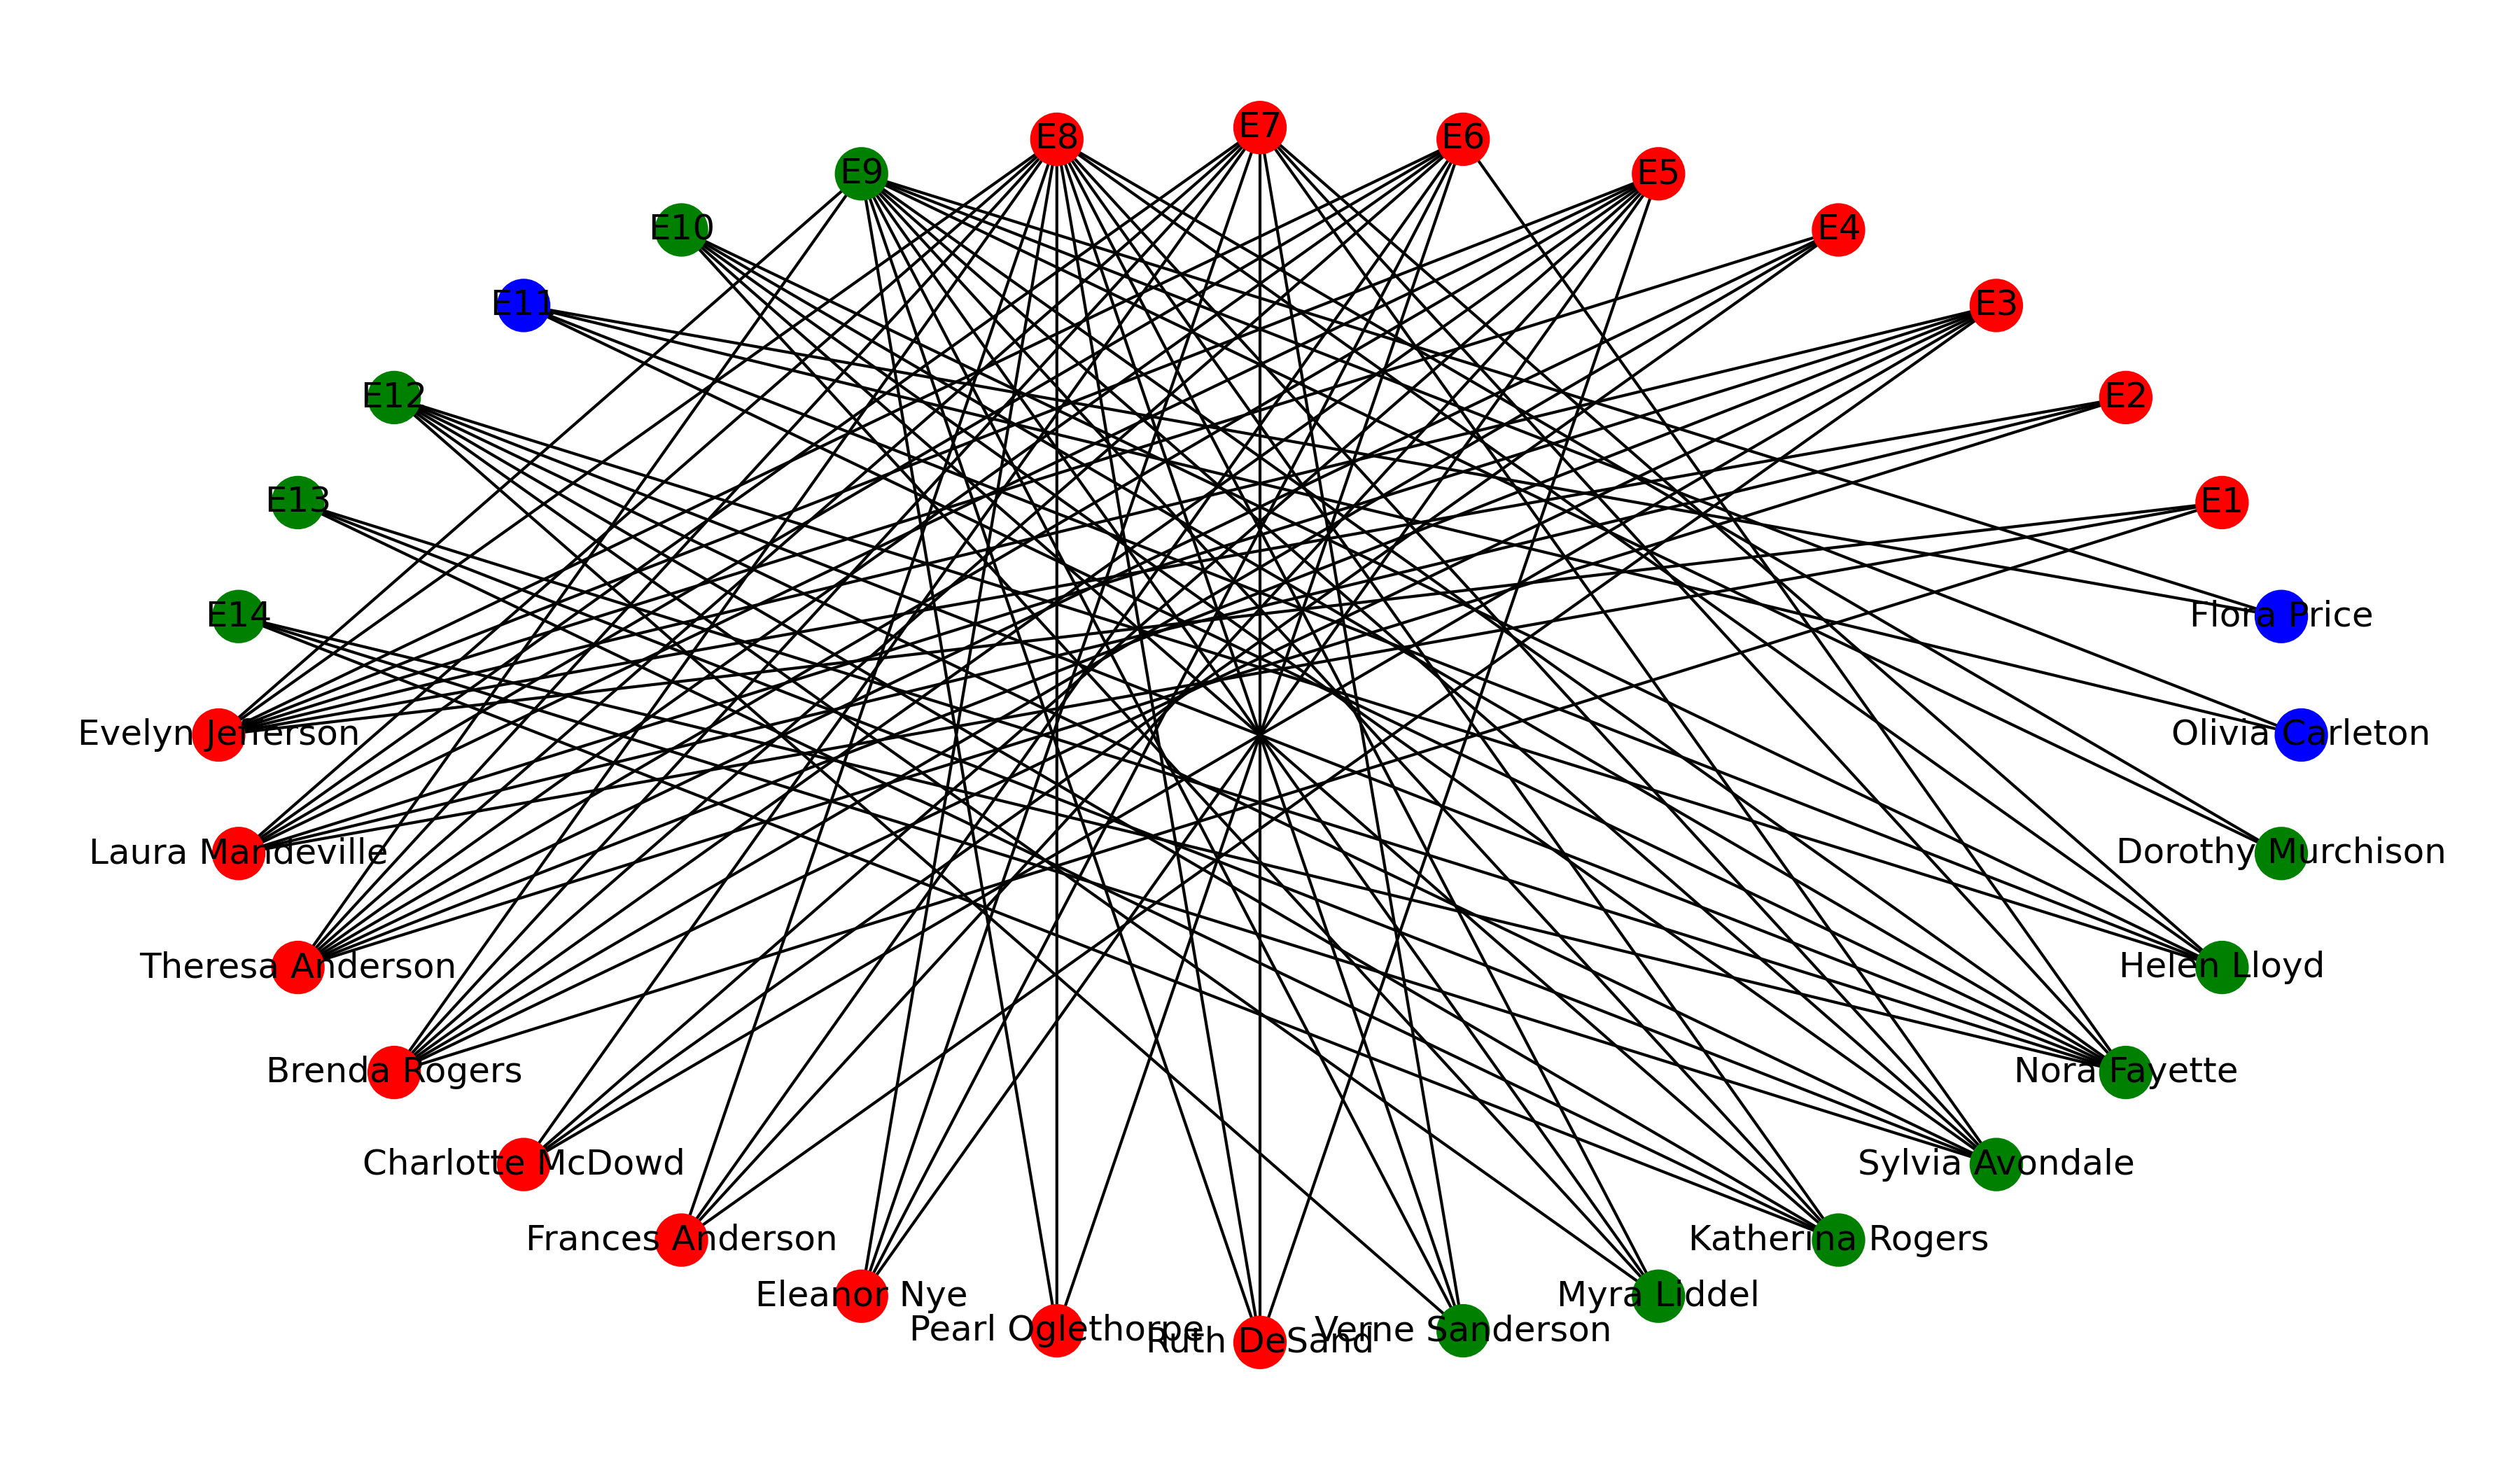
\includegraphics[width=0.8\linewidth]{cluster2.png}
\end{center}
\end{parts}







 
% \question[1--4]{\bf Python/NetworkX questions}:  
% Upload the data regarding the example of bipartite graph  in networkx called the ``Davis Southern Women Graph''
%G = nx.davis\_southern\_women\_graph() 
% . Find:
% \begin{parts}
%\part the graph that link the women that have been in the same social event.
%\part the graph of the social events where one or more guests where the same. 
%\end{parts}



%{\color{blue}\it Hint: 
%The packages that you may need include networkx, matplotlib and numpy. 
%}  

%\begin{center}
%\includegraphics[width=0.5\textwidth]{xx.png}
%\end{center}
\end{questions}
\end{document}



